\section*{Project title: The effects of mindfulness meditation} 
We would like to enquire if you are interested in participating in a 8th semester student project of Biomedical Engineering and Informatics which is to be performed at Aalborg University.
Before you decide to participate in the project, it is important that you fully understand the procedures of the experiment. Therefore, we ask you kindly to read this information carefully.
Participation in the project is voluntary. You can at any time and without stating a reason withdraw your consent.

\section*{Purpose of the experiment}
Previous studies have investigated the usefulness and positive effects of mindfulness meditation on several parts of the daily life.

\section*{Who can participate?}
You can participate in the trial if you fulfill the specific inclusion and exclusion criteria formed for this experiment. 

\textbf{Inclusion criteria:}
	\vspace{-.5cm}
\begin{itemize}
	\item Healthy
	\vspace{-.3cm}
	\item Age between 20 and 40 years
	\vspace{-.3cm}
	\item No obesity 
	\vspace{-.3cm}
	\item Must have time to meditate for 5 days, 20 minutes per day.
\end{itemize}

\textbf{Exclusion criteria:}
	\vspace{-.5cm}
\begin{itemize}
	\item Ongoing meditation practice 
	\vspace{-.3cm}
	\item Pregnancy 
	\vspace{-.3cm}
	\item Neurological, musculoskeletal or mental illness
	\vspace{-.3cm}
	\item Abusive drug or alcohol use
	\vspace{-.3cm}
	\item Medication with antidepressant or analgesic properties
\vspace{-.3cm}
	\item Lack of ability to cooperate
\end{itemize}

Further, you must be able to speak and understand English or Danish.
 
\section*{Experiment}
The experiment consist of two measurement and question sessions, each lasting about 30 minutes. The sessions will be conducted with intervals of approximately one week between them. During the measurement part, we will apply pressure in the right upper trapezius, as illustrated in \figref{fig:trapezius}, with and algometer in order to determine the pressure threshold and the pressure tolerance . 

\begin{figure}[H]
	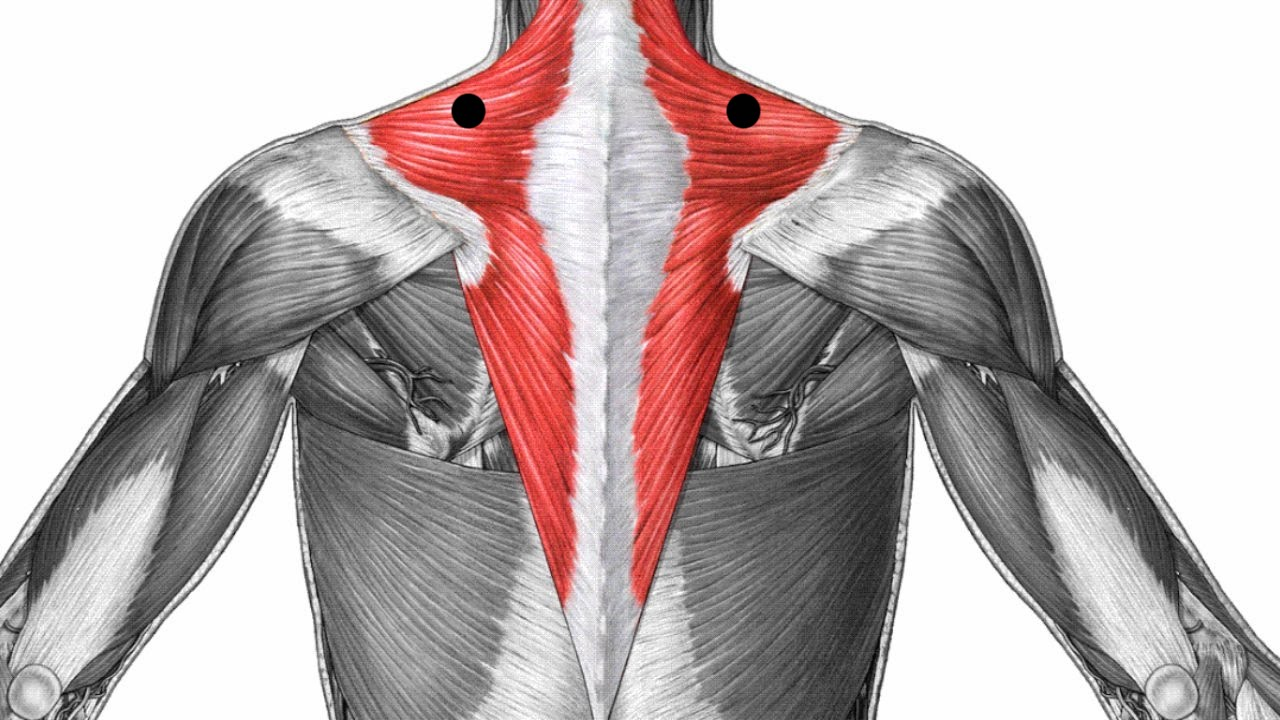
\includegraphics[width=0.5\textwidth]{figures/trapezius.jpg}
	\caption{Measurement points on the upper trapezius}
	\label{fig:trapezius} 
\end{figure}

Between the first and the second measurement and question session, subjects will practice guided mindfulness meditation for 5 consecutive days, each session lasting about 20 minutes. 

\section*{Risk and side effects}
The experimental methods used in this study are well tested and have been used in several studies . No side effects have been reported from these studies.

\section*{Benefits of the experiment}
There will be no immediate personal gain associated with your participation in the trial. However, we expect that the results of the study may contribute to knowledge within the field of mindfulness meditation. Besides the subjects will get an insight in mindfulness meditation and the benefits from practicing it.

\section*{Exclusion from and suspension of experiment}
If the subjects are not suitable for continuing in the experiment the participation can be terminated at any time.
None of the researchers have financial interest in the study.

Contact information:
\textbf{18gr8405@hst.aau.dk or 29475664 and 28244973
}